\documentclass[titlepage, a4paper, 10pt, reqno, openany]{report}
\usepackage{amsfonts}
%\usepackage[brazil]{babel} %linguagem do documento
%\usepackage{babel}
\usepackage[portuguese]{babel}
\usepackage{babelbib}
%\usepackage[utf8]{inputenc} %reconhece acento e cedilha
\usepackage{amssymb}
\usepackage{latexsym}
\usepackage{amsmath}
%\usepackage[fleqn]{amsmath}
%\usepackage{mathtools}
%\usepackage[fleqn]{mathtools}
\usepackage{pxfonts} %permite simbolos matemáticos
\usepackage{mathrsfs} %permite uso de fontes para conjuntos
\usepackage[normalem]{ulem} %permite sublinhar palavras
\usepackage{mathrsfs} %permite o uso de letras trabalhadas
%\usepackage[margin=1in, paperwidth=8.5in, paperheight=11in]{geometry}
%\usepackage[top=1in, bottom=1in, left=1in, right=1in]{geometry}
%\usepackage{fullpage}
\usepackage[top=1.5cm,left=1.5cm,right=1.5cm,bottom=1.5cm]{geometry} %margens
\usepackage{graphicx} %permite inserir figuras
\usepackage[usenames]{color} %permite letras coloridas
\usepackage{makeidx} %pra criar índice remissivo
%\usepackage{tikz}
%\usepackage{pgfplots}
\usepackage{mathptmx}
%\usepackage{named}
\usepackage{enumerate}
%\usepackage{amscls}
%alguns pacotes nao sao reconhecidos, ter atencao quais usar em differents computadores.
\usepackage{float}
\usepackage{caption}
\usepackage{verbatim}
%%%%%%%%%%%%%%%%%%%%
\newtheorem{theorem}{Theorem}
\newtheorem{lemma}{Lemma}
\newtheorem{definition}{Defini\c{c}\~{a}o}
\newtheorem{notation}{Notation}
%%%%%%%%%%%%%%%%%%%%

\bibliographystyle{babplain}

\makeindex

\begin{document}
\renewcommand\thesection{\arabic{section}}
\renewcommand\thesubsection{\thesection.\arabic{subsection}}
\renewcommand\thesubsubsection{\thesection.\thesubsection.\arabic{subsubsection}}
\pagestyle{plain}%plain headings empty
%%%%%%%%%%%%%%%%%%%%%%%%%%%%%%%%%%%%%%%%%%%%%%%%%%%%%%%%%%%%%%%%%%%%%%%%%%%%
\chapter*{Trabalho 3 Prep}
{\bf Nome: Sérgio Santos} \\
\hspace*{0.51cm}{\bf nº: 1020881}\\
\section{Esquema}
\begin{figure}[H]
	\centering
	\includegraphics[scale=0.6]{./image/esquema.jpg}\\
	\caption{Esquema}
\end{figure}
Um condensador quando esta a ser alimentado por uma fonte de corrente com um valor constante este carrega de forma linear no tempo, sendo que a corrente fornecida determina sua taxa de crescimentos, $\left[ \frac{Volt}{Sec} \right]$.\\ \\
O circuito alimentado com uma fonte de 19 Volt tem tensão mínimo e máximo: \\
\begin{minipage}[l]{0pt}
	$$\left\lbrace\begin{array}{c}
 	-8,4 \quad V \\
 	9 \quad V \\
 \end{array}\right.$$
\end{minipage}
\hspace{3cm} 12,9 Kohm \hspace{3cm}
\begin{minipage}[l]{0pt}
	$$\left\lbrace\begin{array}{c}
		6,5116 \times 10^{-4} \quad A \\
		6,9767 \times 10^{-4} \quad A \\
	\end{array}\right.$$
\end{minipage}\\
\\
\\
Vamos ver que o integrador vai usar um condensador de 1nF, que vai necessitar de uma corrente de carga de $6,96 \times 10^{-4} \quad A$, na qual traduz na resistência a ser usada, já que a malha de realimentação é uma fonte de corrente determinada pela resistência colocada na entrada inversor, é o principio de funcionamento do {\bf AMPOP} com realimentação negativa, mantém as entradas sempre ao mesmo potencial.
\begin{figure}[H]
	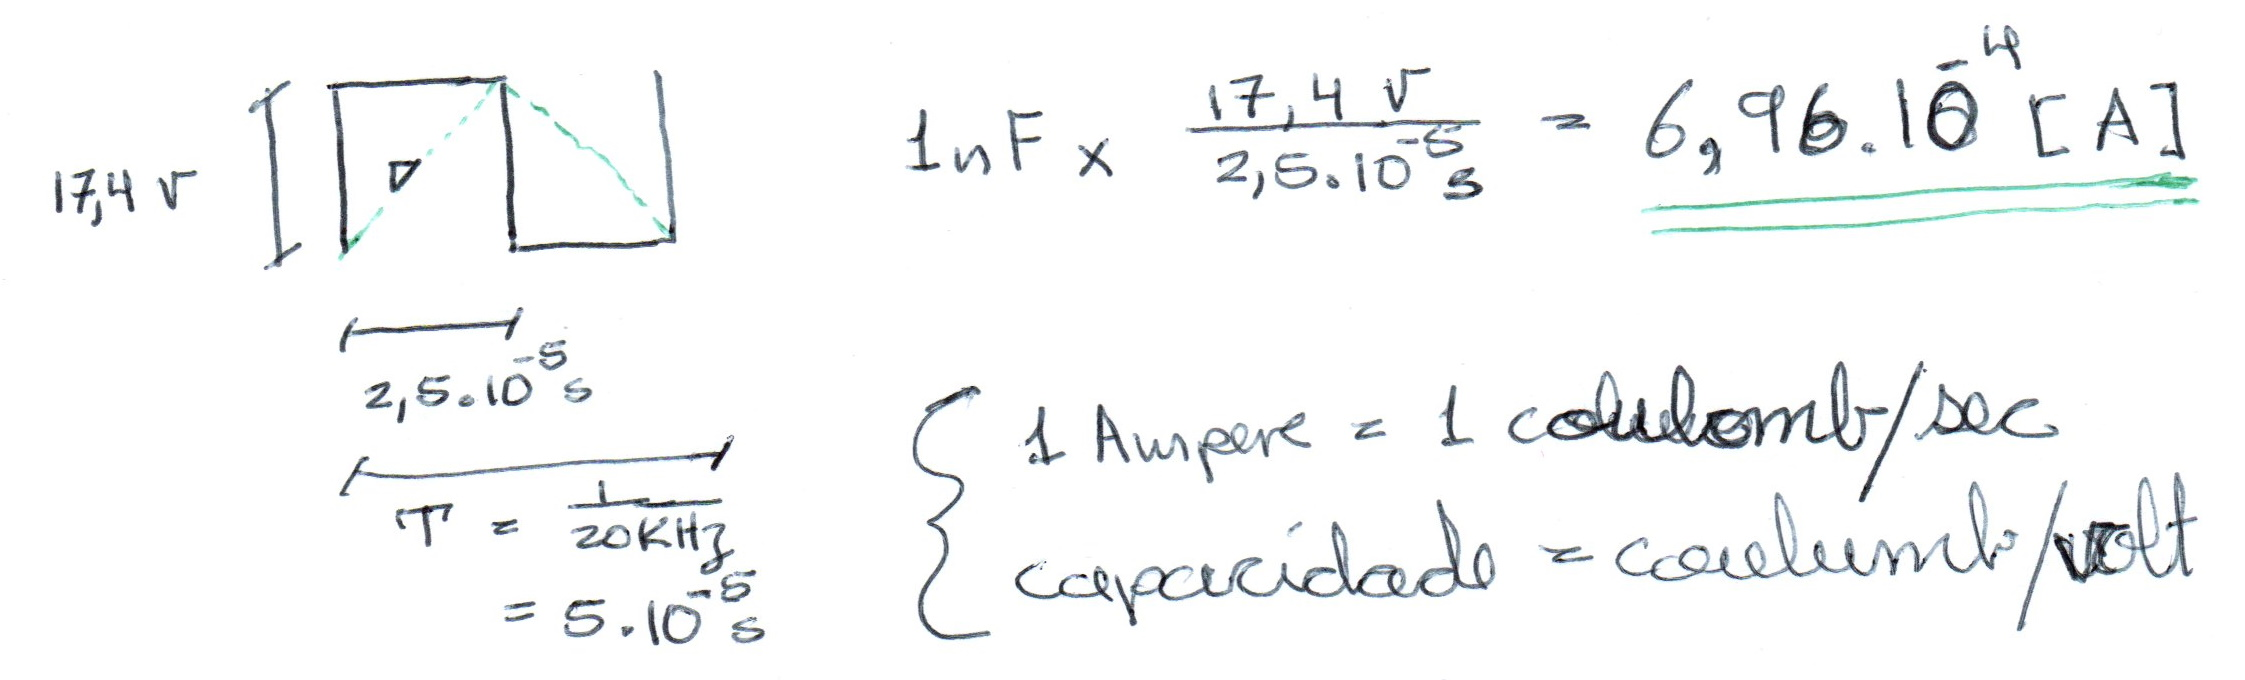
\includegraphics[scale=0.9]{./image/trb3calc_1.jpg}\\
	\caption{Determinar Corrente}
\end{figure}
%%%%%%%%%%%%%%%%%%%%%%%%%%%%%%%%%%%%%%%%%%%%%%%%%%%%%%%%%%%%%%%%%%%%%%%%%%%
\section{Material}
\begin{minipage}[t]{.4\linewidth}
	\begin{itemize}
		\setlength\itemsep{-0.5em}
		\item Resistencias \\
		1/4 Watt, varias.
		\item Potenciómetro multi-volta \\
		100Kohm e 1Kohm
		\item Condensador \\
		1nF, 10nF  \\
		2x Eletrolítico 10uF
		
	\end{itemize}
\end{minipage}
\begin{minipage}[t]{.31\linewidth}
	%	\quad List 2:
	\begin{itemize}
		\setlength\itemsep{-0.5em}
		\item TL084 \\
		Quad Opamp Chip \\
		14 Pinos
		\item Ficha Alimentação
		\item Fusível 800mA
		\item Diodo 1N4148
		\item Led Verde \\
	\end{itemize}
\end{minipage}\\
\\
Circuito Funciona de 10 Volt até 32 Volt testado em bancada, sendo necessário ajuste fino para calibração pelo Potenciómetro de  1Kohm.
Pode se sempre consultar os {\it datasheets} dos componentes.
\section{PCB (Printed Circuit Board)}
%\begin{comment}	
\begin{figure}[ht]
\begin{center}
	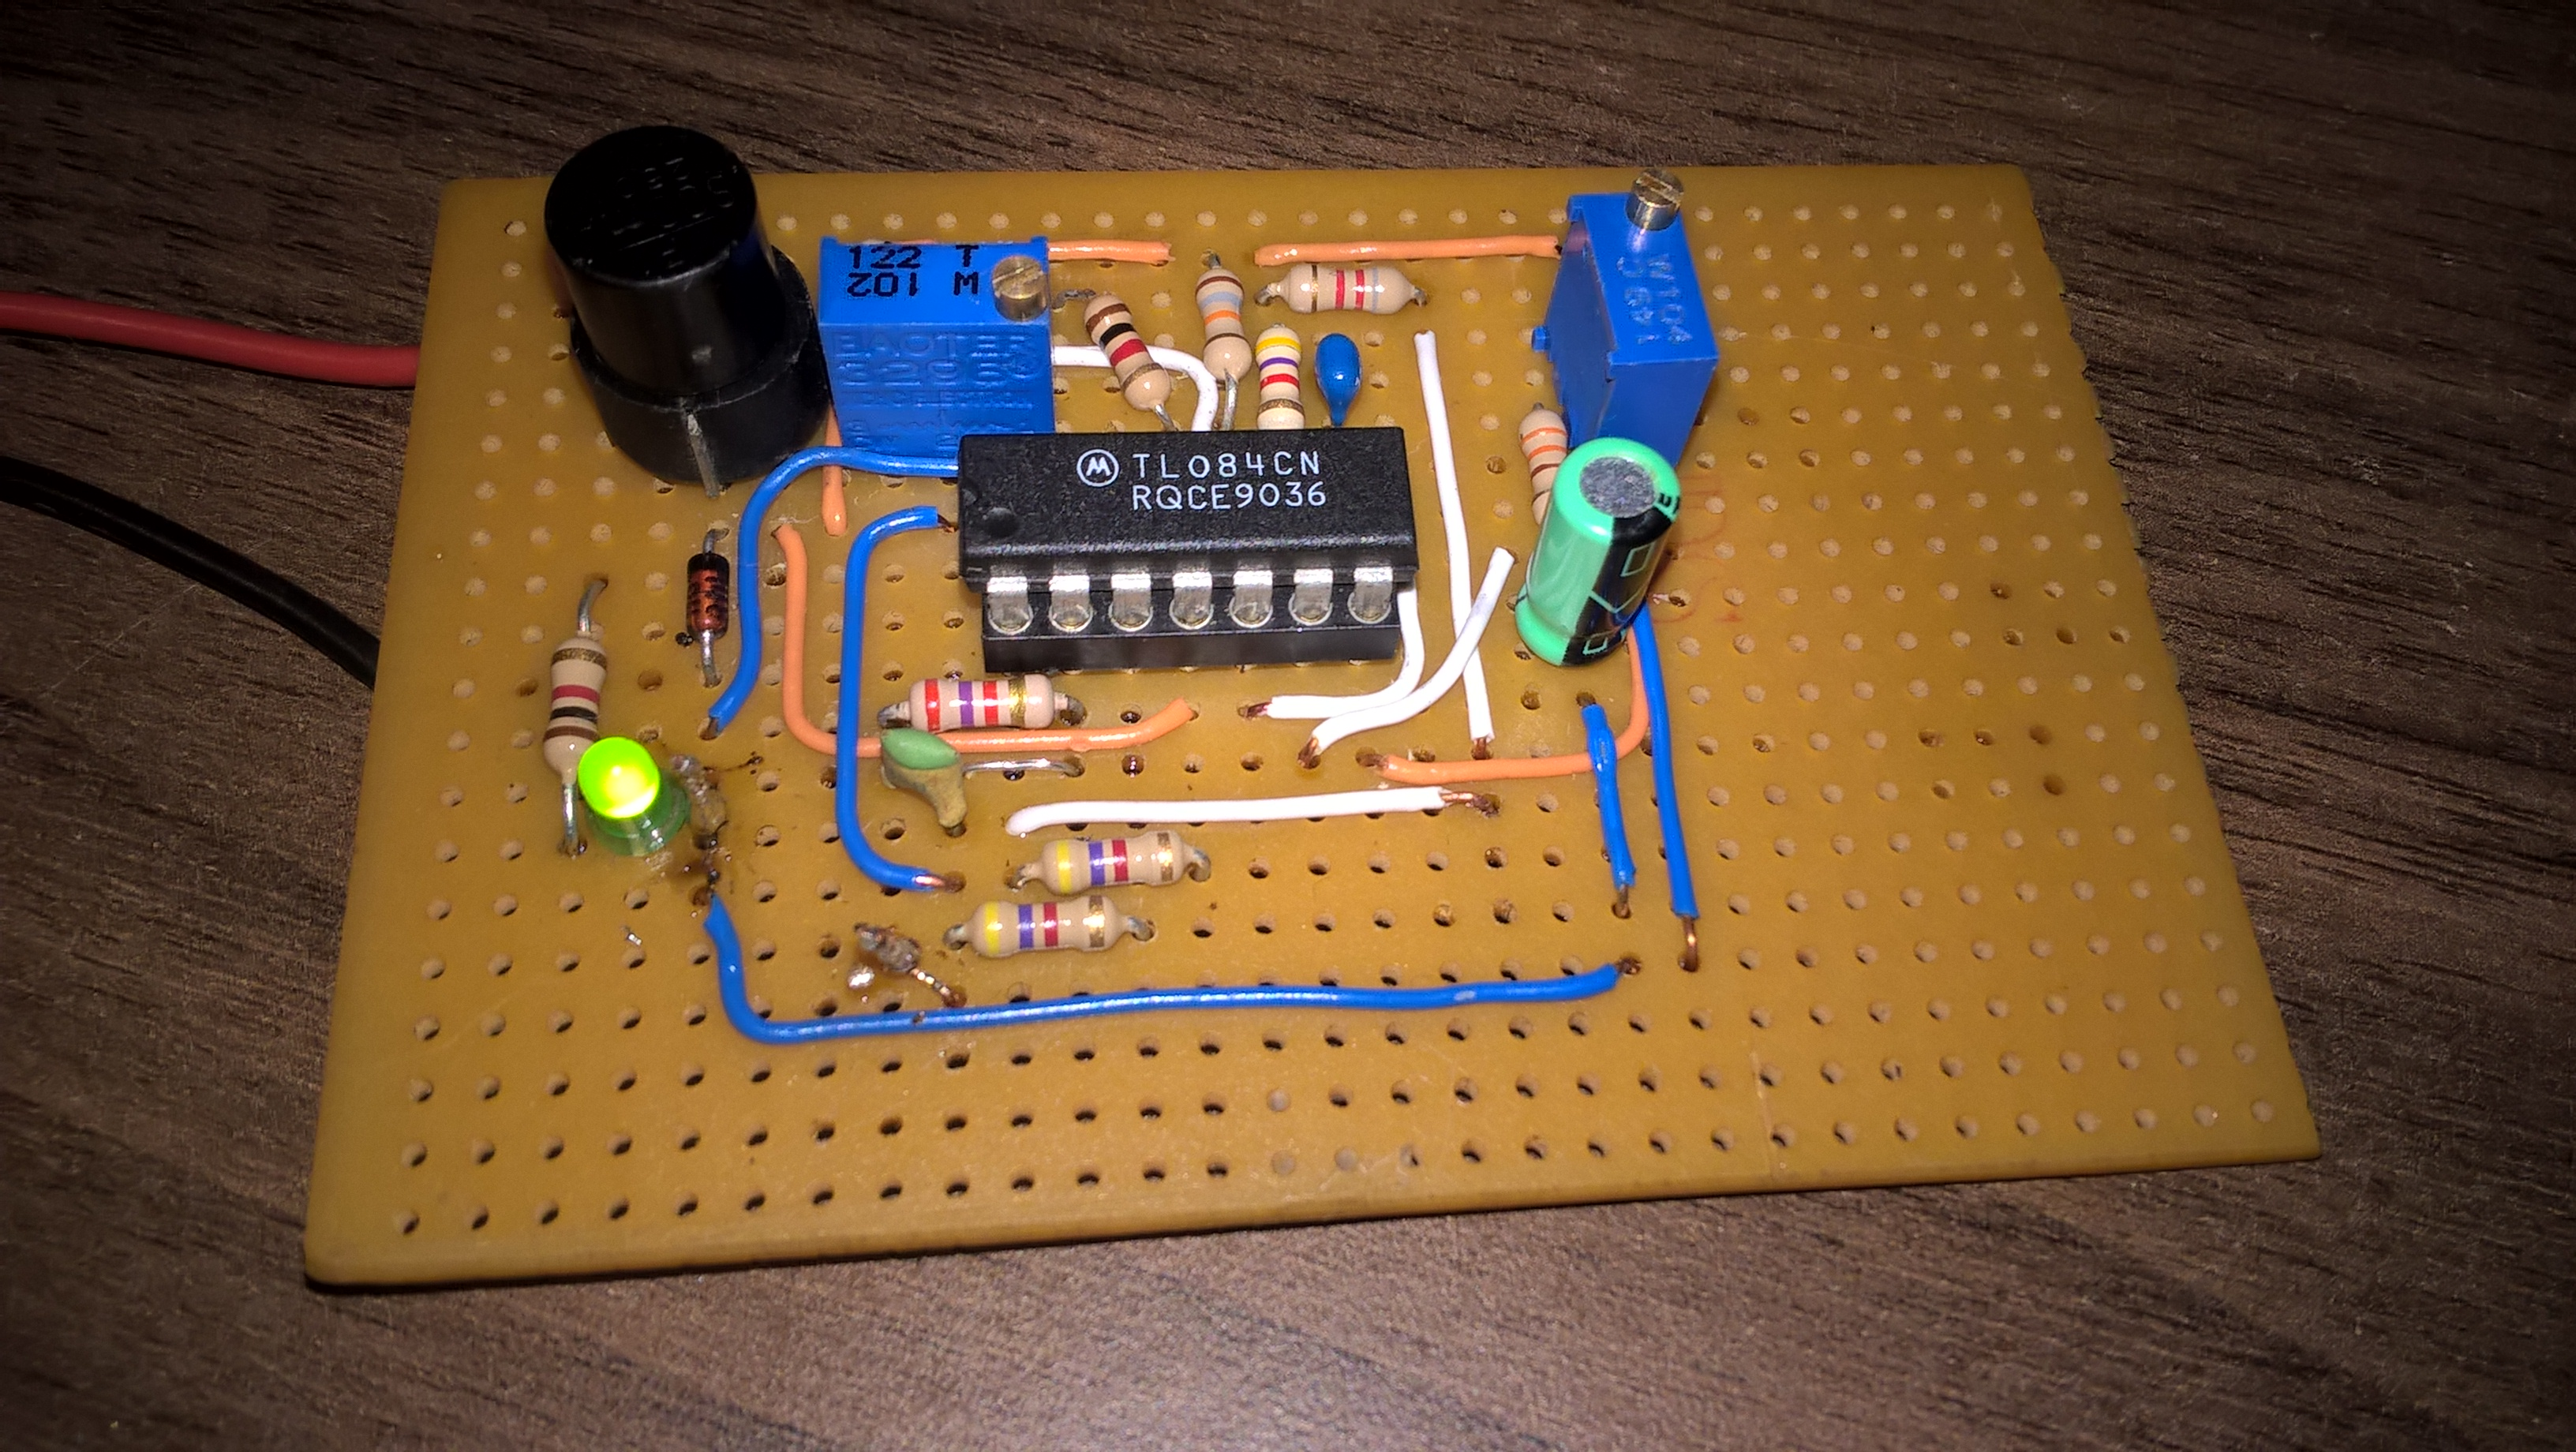
\includegraphics[scale=0.07]{./image/placa_1.jpg} \hspace{0.2cm}
	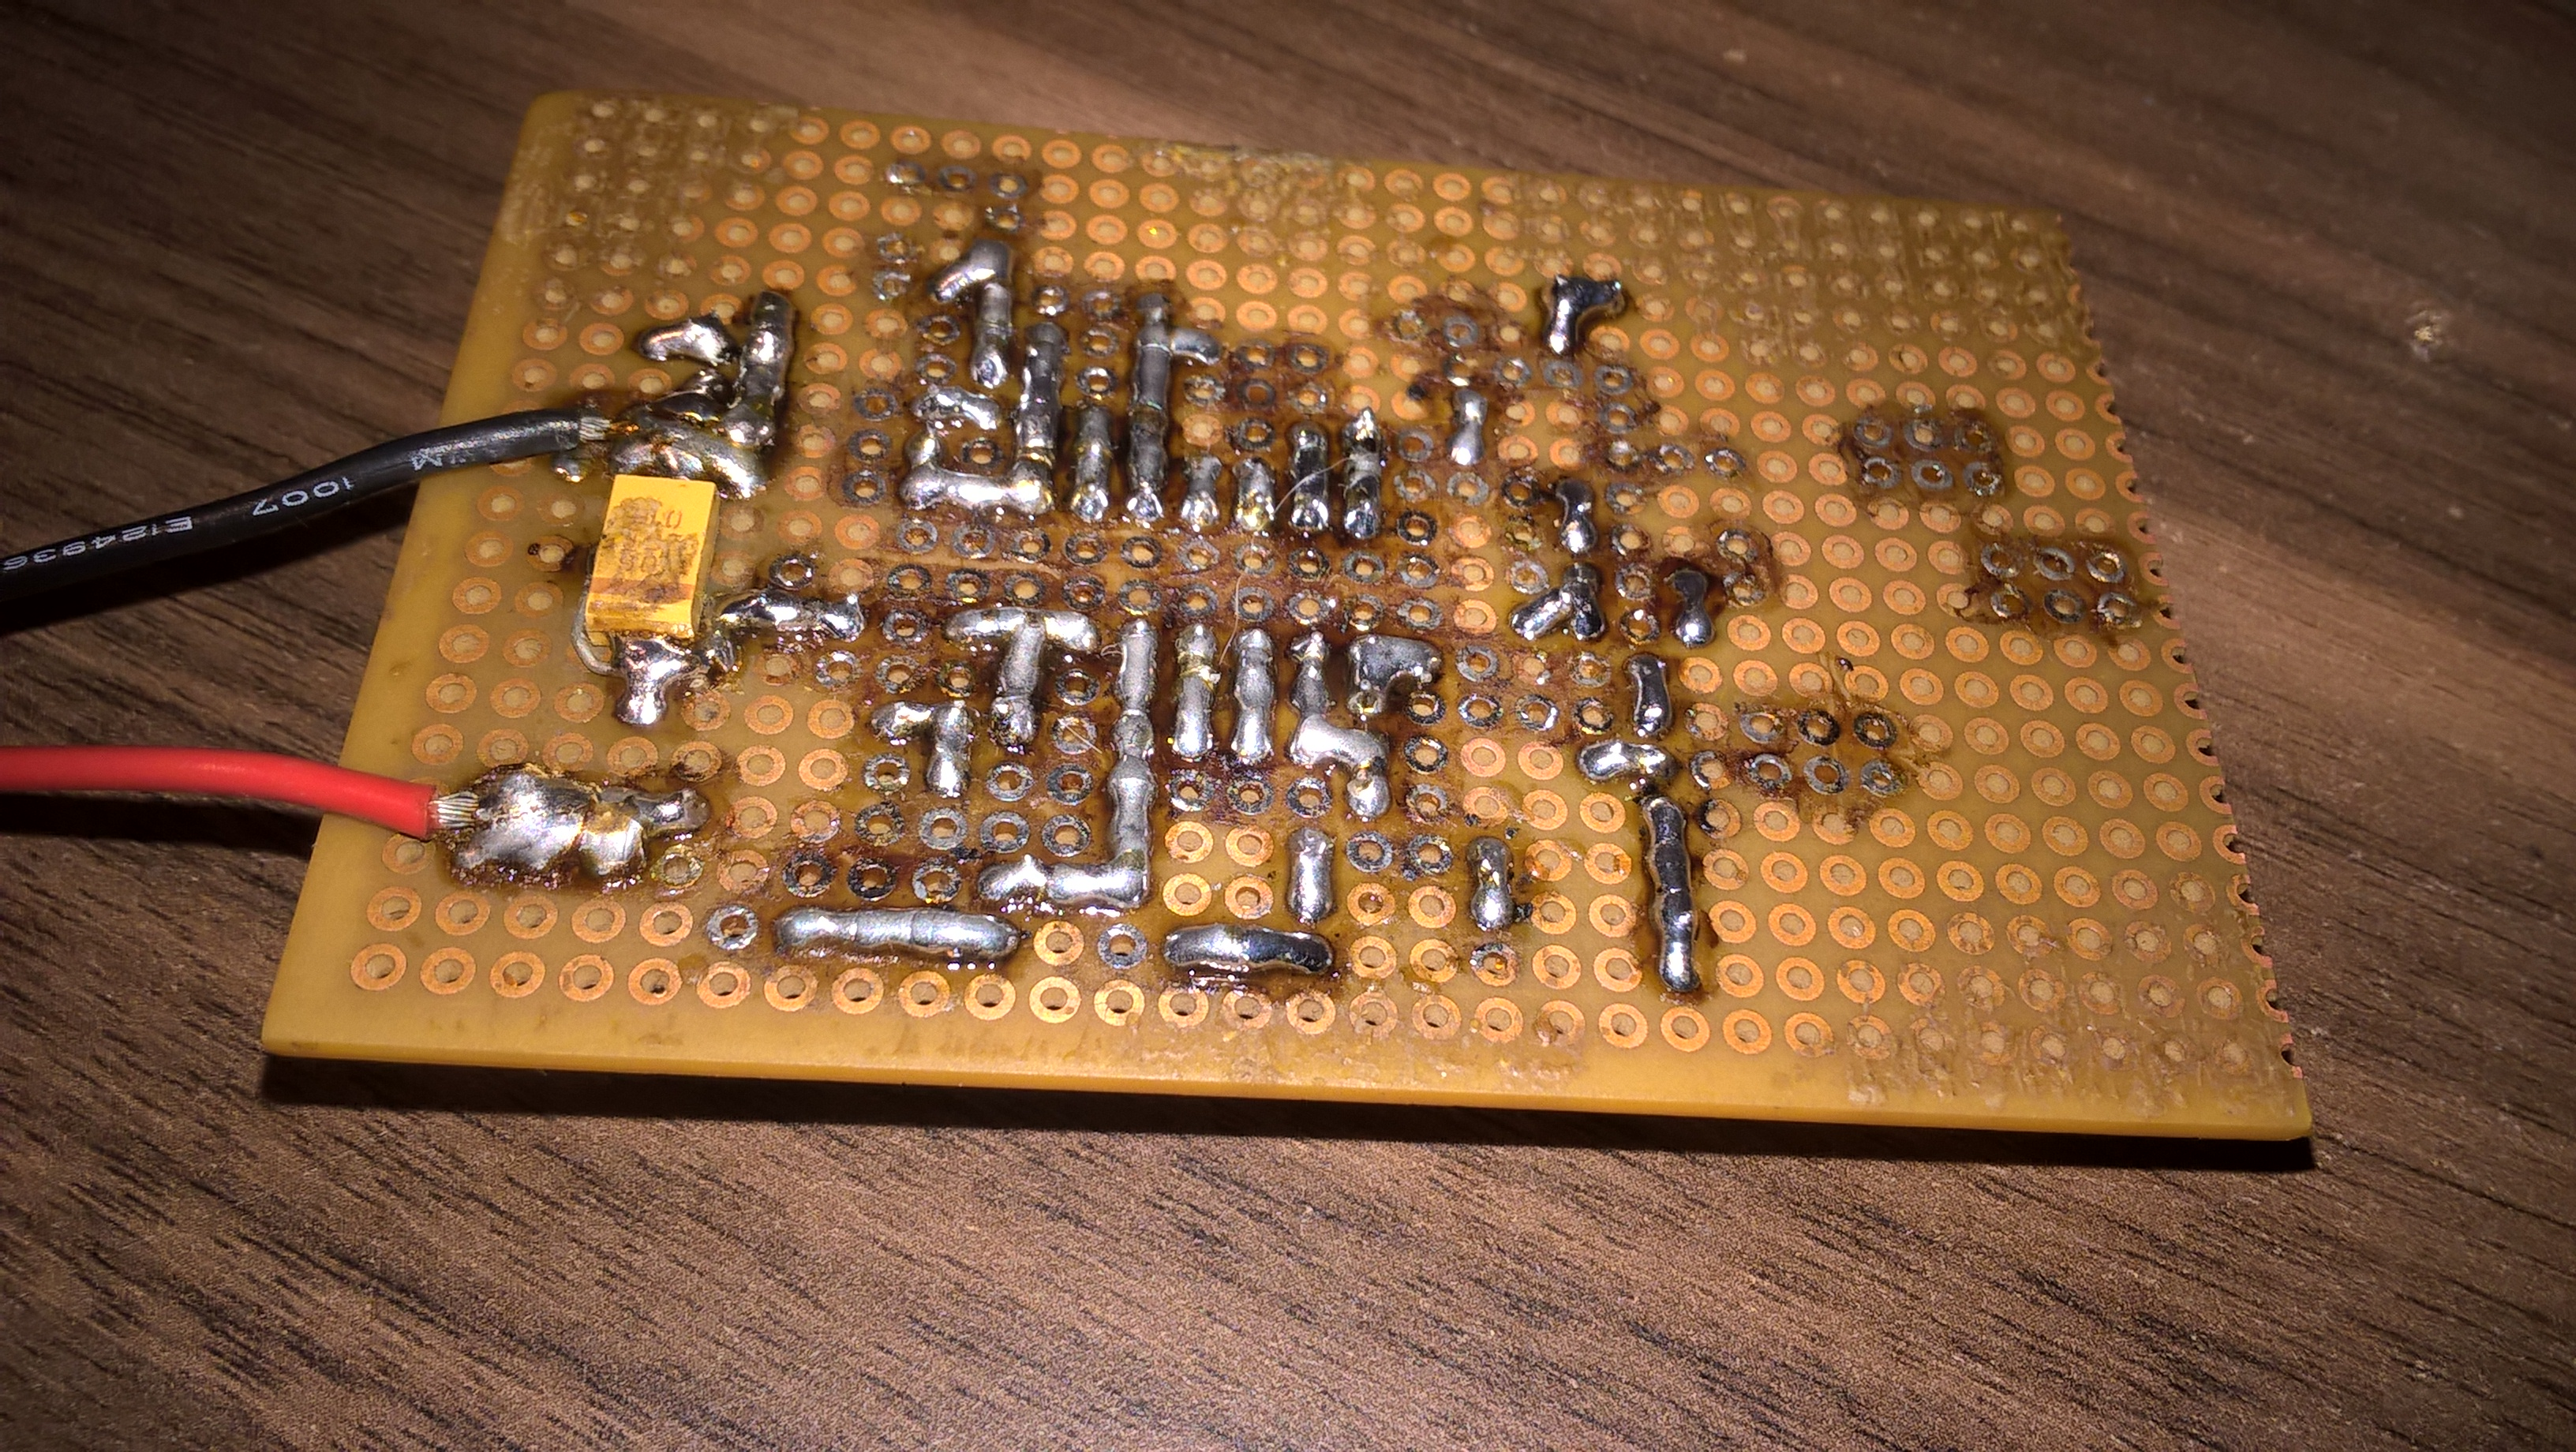
\includegraphics[scale=0.07]{./image/placa_2.jpg}
\end{center}
\caption{PCB}
\end{figure}\par
Este circuito tem um comportamento muito estável e flexibilidade, temos de ter em conta as características dos componentes, que não interfere na sua funcionalidade mas na tolerância que é dependente da temperatura, alimentação e dos componentes, se se quer grande precisão só através de medição e ajustes.
%%%%%%%%%%%%%%%%%%%%%%%%%%%%%%%%%%%%%%%%%%%%%%%%%%%%%%%%%%%%%%%%%%%%%%%%%%%
\section{Simulação}
%\begin{comment}	
\begin{figure}[H]
	\centering
	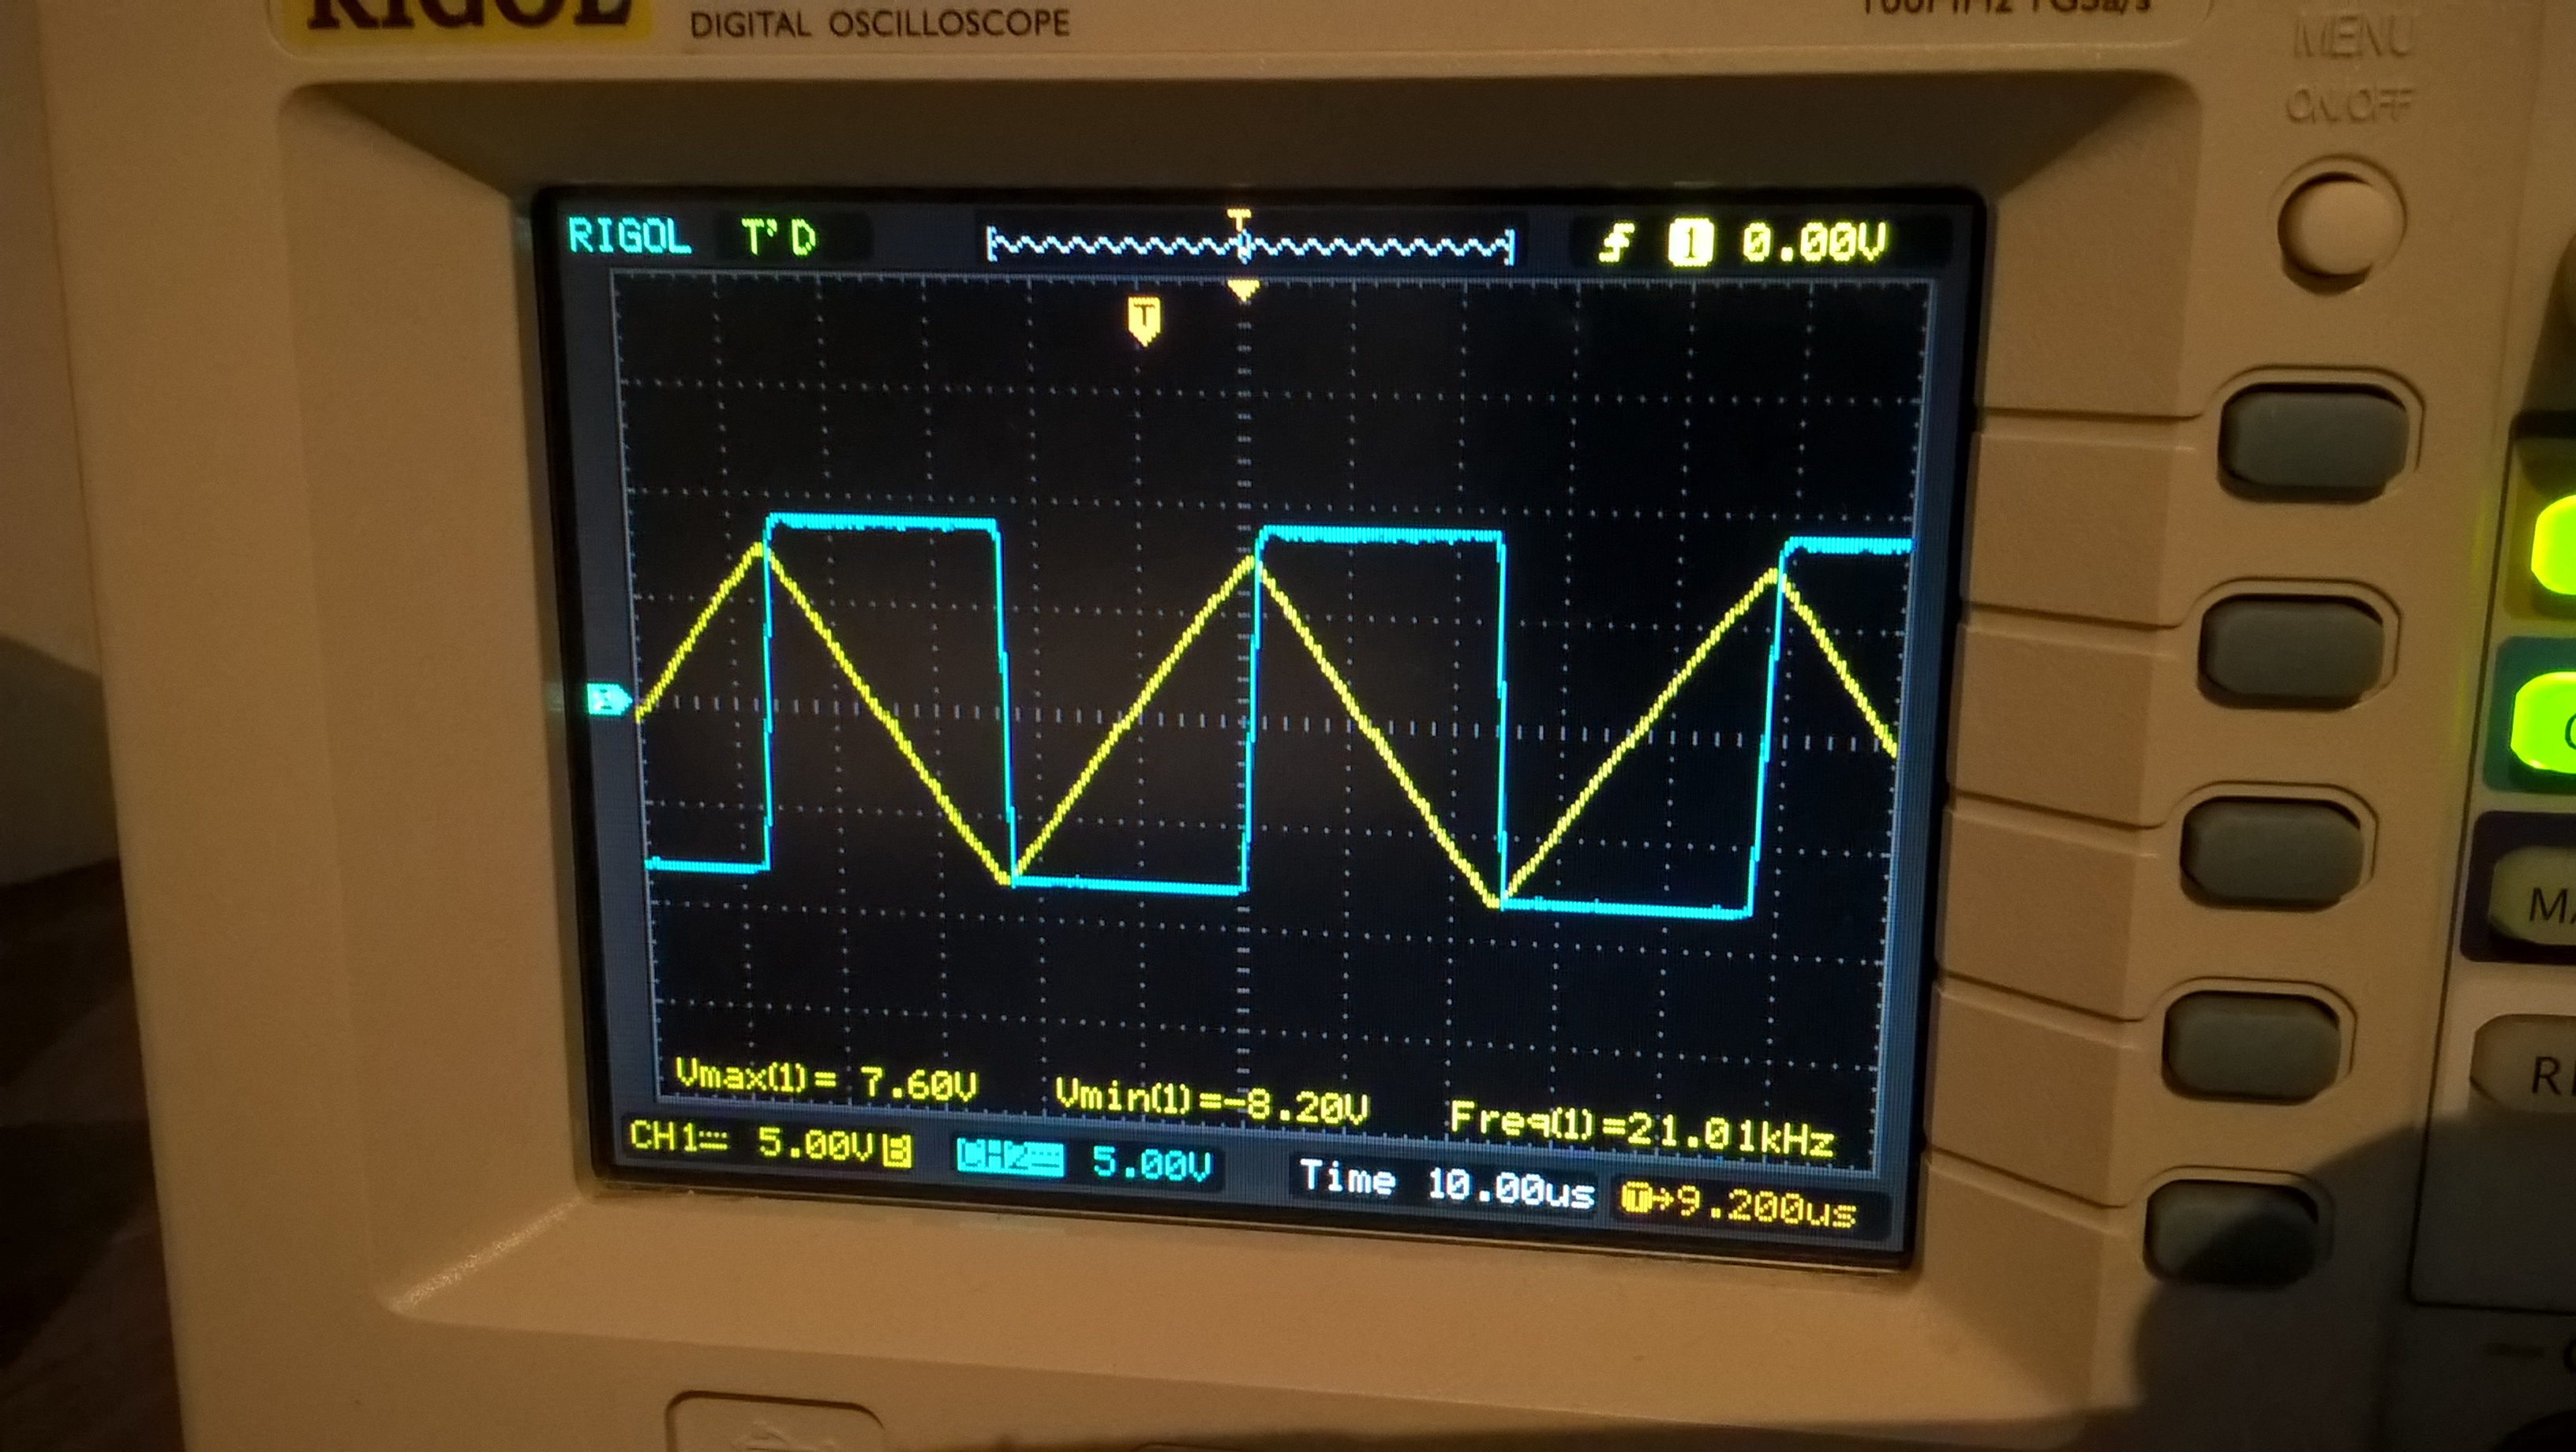
\includegraphics[scale=0.13]{./image/Ondas.jpg}\\
	\caption{Ondas}
\end{figure}
%\end{comment}
\newpage
%%%%%%%%%%%%%%%%%%%%%%%%%%%%%%%%%%%%%%%%%%%%%%%%%%%%%%%%%%%%%%%%%%%%%%%%%%%
\newpage
\footnote{Apontamentos}
%
	\end{document}
%%%%%%%%%%%%%%%%%%%%%%%%%%%%%%%%%EOF%%%%%%%%%%%%%%%%%%%%%%%%%%%%%%%%%%%%%%%
\begin{comment}
\begin{figure}[H]
\centering
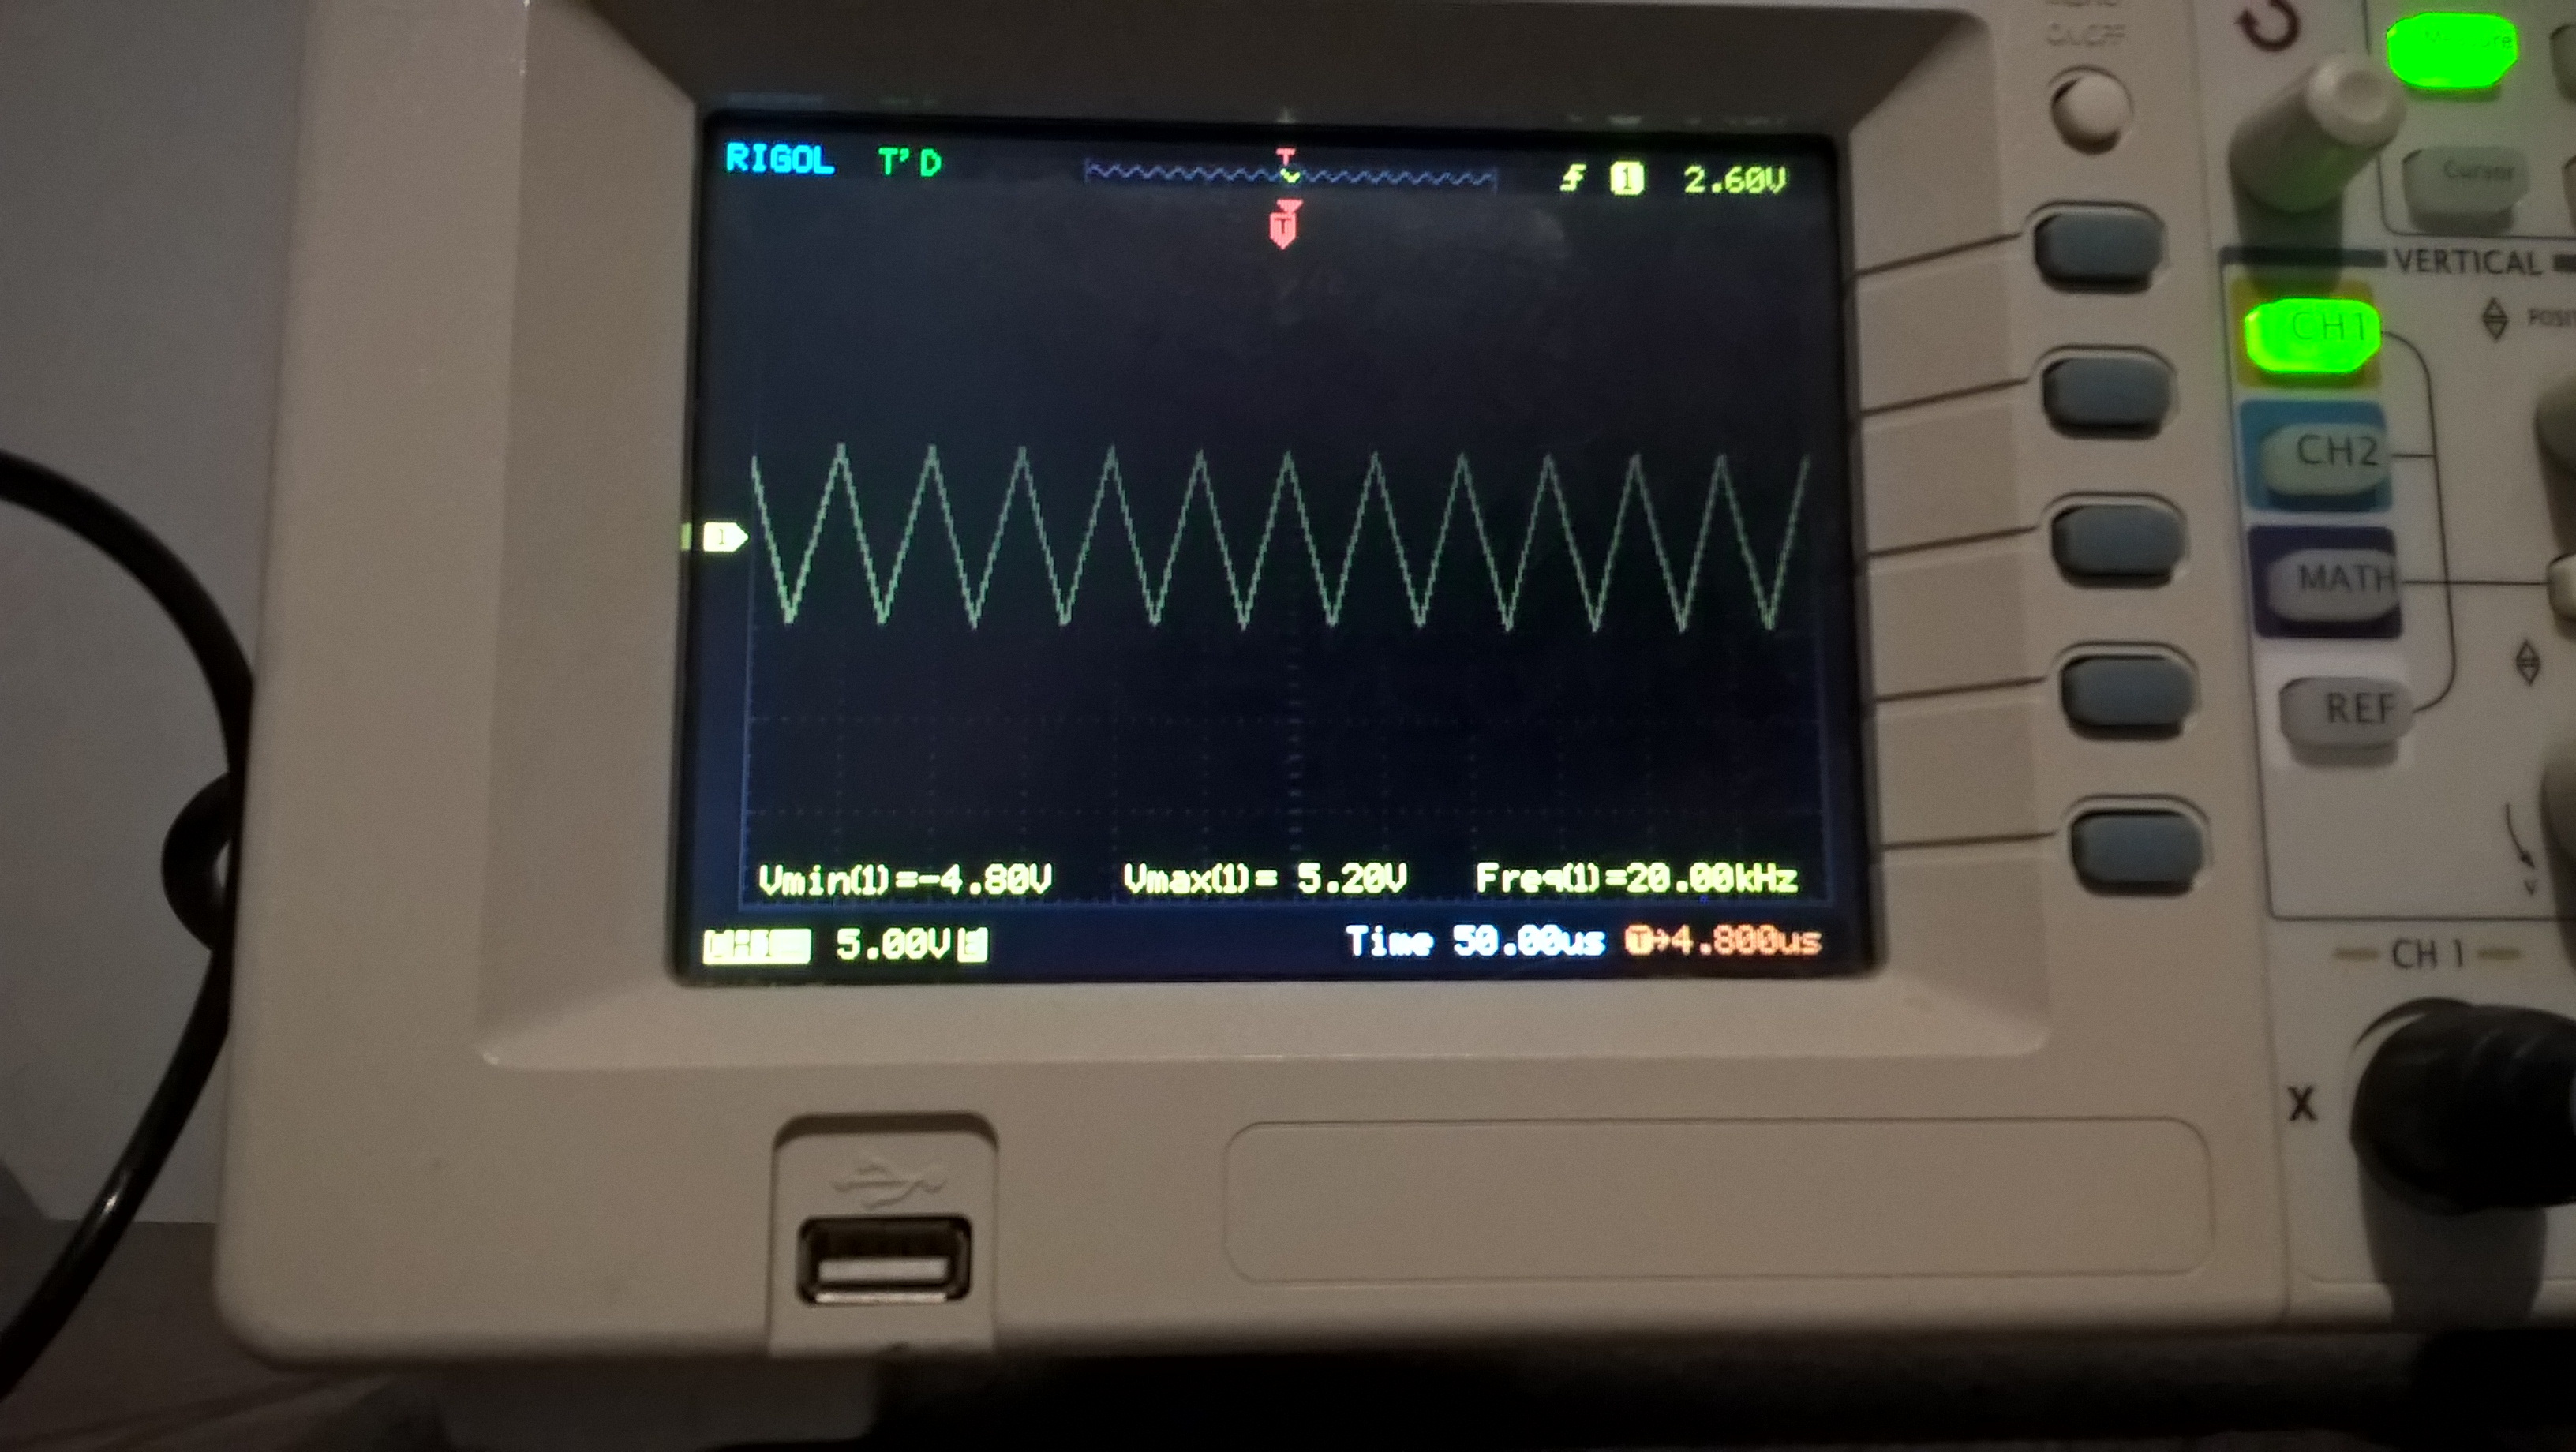
\includegraphics[scale=0.15]{./image/triangulo.jpg}\\
\caption{Onda Triangular}
\end{figure}\par
\end{comment}
%%%%%%%%%%%%%%%%%%%%%%%%%%%%%%%%%%%%%%%%%%%%%%%%%%%%%%%%%%%%%%%%%%%%%%%%%%%%